\documentclass{article}
\usepackage{algorithm,algorithmic}
\usepackage{amsmath}
\usepackage{amsthm}
\usepackage{amssymb}
\usepackage{enumerate}
\usepackage[margin=1.00in]{geometry}
\usepackage{graphicx}
\usepackage{hyperref}
\usepackage{tikz}

% new theorems
\newtheorem{theorem}{Theorem}[section]
\newtheorem{proposition}[theorem]{Proposition}
\newtheorem{corollary}[theorem]{Corollary}
\newtheorem{example}[theorem]{Example}

% indent for algorithm pseudo-code
\newlength\myindent
\setlength\myindent{1em}
\newcommand\bindent{%
  \begingroup
  \setlength{\itemindent}{\myindent}
  \addtolength{\algorithmicindent}{\myindent}
}
\newcommand\eindent{\endgroup}

% new commands and math operators
\newcommand*\conj[1]{\overline{#1}}
\newcommand{\iu}{{i\mkern1mu}}
\newcommand\abs[1]{\left|#1\right|}
\newcommand\norm[1]{\left\Vert#1\right\Vert}
\newcommand\diag[1]{\operatorname{diag}\left(#1\right)}
\newcommand\re[1]{\operatorname{Re}\left(#1\right)}
\newcommand\sv[2]{\operatorname{sv}_{#1}(#2)}
\newcommand\hd[2]{\operatorname{hd}(#1,#2)}
\newcommand\md[2]{\operatorname{md}(#1,#2)}
\newcommand\func[1]{\operatorname{function}~[#1]}
\DeclareMathOperator{\specr}{SpecR}
\DeclareMathOperator{\ipr}{IPR}



\title{A Note to Panos:\\
\emph{\large{Algebraic Connectivity of Perfect Dominance Graphs}}}
\author{Thomas R. Cameron}
\date{\today}

\begin{document}
\maketitle
\abstract{
This note is an introduction to a wonderful connection between the algebraic connectivity of a graph, the field of values of a matrix, and the rankability of data. 
}

%%%%%%%%%%%%%%%%%%%%%%%%%%%%%%%%%%%%%%%%%%%%%%%%%%%%%%
%                                    				Introduction
%%%%%%%%%%%%%%%%%%%%%%%%%%%%%%%%%%%%%%%%%%%%%%%%%%%%%%
\section{Introduction}	
Recently, the problem of rankability of posed, which refers to a dataset's inherent ability to produce a meaningful ranking of its items~\cite{Anderson2018}.
Given data that can be modeled as a binary directed graph, the idea is to measure how far that graph is from a \emph{perfect dominance graph}, i.e., an acyclic tournament graph.
A perfect dominance graph represents an ideal situation for ranking as it is associated with a clear and unique ranking, e.g.,
the perfect dominance graph associated with the ranking $[1,2,3,4,5,6]$ is shown in Figure~\ref{fig:dom}.

%%%%%%%%%%%%%%%%%%%%%%
%			Figure 1				%
%%%%%%%%%%%%%%%%%%%%%%
\begin{figure}[ht]
\centering
\resizebox{0.18\textwidth}{!}{% Perfect Dominance
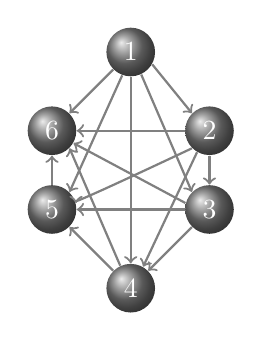
\begin{tikzpicture}
	\node[circle, shading=ball, ball color=gray, color=white] (1) at (0,2) {$1$};
	\node[circle, shading=ball, ball color=gray, color=white] (2) at (1,1) {$2$};
	\node[circle, shading=ball, ball color=gray, color=white] (3) at (1,0) {$3$};
	\node[circle, shading=ball, ball color=gray, color=white] (4) at (0,-1) {$4$};
	\node[circle, shading=ball, ball color=gray, color=white] (5) at (-1,0) {$5$};
	\node[circle, shading=ball, ball color=gray, color=white] (6) at (-1,1) {$6$};
	
	% vertex 1
	\draw[gray,->,thick](1) to [out=330,in=135,looseness=0](2);
	\draw[gray,->,thick](1) to [out=295,in=135,looseness=0](3);
	\draw[gray,->,thick](1) to [out=270,in=90,looseness=0](4);
	\draw[gray,->,thick](1) to [out=250,in=45,looseness=0](5);
	\draw[gray,->,thick](1) to [out=225,in=45,looseness=0](6);
	% vertex 2
	\draw[gray,->,thick](2) to [out=270,in=90,looseness=0](3);
	\draw[gray,->,thick](2) to [out=240,in=60,looseness=0](4);
	\draw[gray,->,thick](2) to [out=225,in=15,looseness=0](5);
	\draw[gray,->,thick](2) to [out=180,in=0,looseness=0](6);
	% vertex 3
	\draw[gray,->,thick](3) to [out=225,in=45,looseness=0](4);
	\draw[gray,->,thick](3) to [out=180,in=0,looseness=0](5);
	\draw[gray,->,thick](3) to [out=165,in=330,looseness=0](6);
	% vertex 4
	\draw[gray,->,thick](4) to [out=135,in=315,looseness=0](5);
	\draw[gray,->,thick](4) to [out=115,in=315,looseness=0](6);
	% vertex 5
	\draw[gray,->,thick](5) to [out=90,in=270,looseness=0](6);
	% vertex 6
\end{tikzpicture}%
}
\caption{Perfect dominance graph associated with ranking $[1,2,3,4,5,6]$.}
\label{fig:dom}
\end{figure}

Now, in theory, the rankability measure proposed in~\cite{Anderson2018} is simple.
Let $k$ denote the minimum number of edge deletions or additions made to the given graph in order to obtain a perfect dominance graph.
Given $k$ edge changes, denote by $p$ the number of perfect dominance graphs that can be obtained.
Then, the rankability measure of the given dataset is defined by
\begin{equation}\label{eq:simod-rank}
\ipr = 1 - \frac{kp}{k_{max}p_{max}},
\end{equation}
where $k_{max}=(n^{2}-n)/2$ and $p_{max}=n!$.
We denote this rankability measure by $\ipr$ since an integer program is used to compute $k$ and $p$. 

This rankability measure is clearly expensive to compute (in fact, I believe it is NP Hard).
Therefore, even more recently, we proposed a cheaper rankability measure, which is motivated by a spectral-degree characterization of perfect dominance graphs.

%%%%%%%%%%%%%%%%%%%%%%
%			Theorem 1.1			%
%%%%%%%%%%%%%%%%%%%%%%
\begin{theorem}[See Corollary 2.9 of Pre-Print]
Let $\Gamma\in\mathbb{G}$ have binary weights and let $L$ be the graph Laplacian of $\Gamma$.
Then, $\Gamma$ is a perfect dominance graph if and only if 
\[
\sigma(L)=\left\{d^{+}(1),\ldots,d^{+}(n)\right\}
\]
and there exists a re-ordering of the vertices such that $d^{+}(i)=n-i$ for $i=1,\ldots,n$. 
\end{theorem}

Armed with this spectral-degree characterization, we propose the following measure of the rankability of data.
Note that $\hd$ denotes the Hausdorff distance and the maximum upper bound for both $\hd{D}{S}$ and $\hd{L}{S}$ is $(n-1)$.
Therefore, the division by $2(n-1)$ is a normalization factor.
Finally, note that $r$ ranges between $0$ and $1$, which indicates a transition between ill-rankable and well-rankable data. 

%%%%%%%%%%%%%%%%%%%%%%
%			Algorithm 1			%
%%%%%%%%%%%%%%%%%%%%%%
\begin{algorithm}[ht]
\caption{Spectral Rankability of Graph Data $\Gamma$.}
\label{alg:specr}
\begin{algorithmic}
\STATE{$\func{r} = \specr\left(\Gamma\right):$}
\bindent
\STATE{$n\gets$ the number of vertices in $\Gamma$}
\STATE{$D\gets$ the out-degree matrix of $\Gamma$}
\STATE{$L\gets$ graph Laplacian of $\Gamma$}
\STATE{$S=\diag{n-1,n-2,\ldots,0}$}
\STATE{$r=1 - \frac{\hd{D}{S}+\hd{L}{S}}{2(n-1)}$}
\RETURN
\eindent
\end{algorithmic}
\end{algorithm}

In Figure~\ref{fig:simod-examples}, we consider several examples from~\cite{Anderson2018}, which tests whether a rankability measure aligns with our intuitive classification of certain structured datasets as well-rankable or ill-rankable.
For each dataset, we compare $\specr$ with the measure $\ipr$ as defined in~\eqref{eq:simod-rank}.

Note that the graphs are displayed from most rankable to least rankable as determined by the measure $\ipr$.
The measures $\specr$ and $\ipr$ have a strong correlation, the Pearson correlation coefficient between them is $0.92$. 
In addition, the measures $\specr$ and $\ipr$ have exact agreement on the extreme cases, i.e., the perfect dominance graph and empty graph.
Finally, if the matching distance is used to measure the variation, then there is also exact agreement on the completely connected graph, and the Pearson coefficient is $0.94$.


%%%%%%%%%%%%%%%%%%%%%%
%			Figure 2				%
%%%%%%%%%%%%%%%%%%%%%%
\begin{figure}[ht]
\centering
\resizebox{0.9\textwidth}{!}{%
\begin{tabular}{cccc}
\textbf{Perfect Dominance} & \textbf{Perturbed Dominance} & \textbf{Perturbed Random} & \textbf{Nearly Disconnected} \\
\resizebox{0.2\textwidth}{!}{% Perfect Dominance
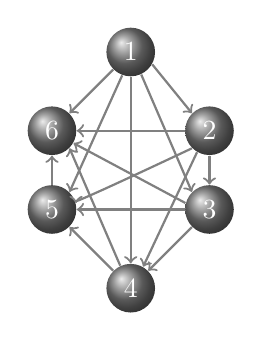
\begin{tikzpicture}
	\node[circle, shading=ball, ball color=gray, color=white] (1) at (0,2) {$1$};
	\node[circle, shading=ball, ball color=gray, color=white] (2) at (1,1) {$2$};
	\node[circle, shading=ball, ball color=gray, color=white] (3) at (1,0) {$3$};
	\node[circle, shading=ball, ball color=gray, color=white] (4) at (0,-1) {$4$};
	\node[circle, shading=ball, ball color=gray, color=white] (5) at (-1,0) {$5$};
	\node[circle, shading=ball, ball color=gray, color=white] (6) at (-1,1) {$6$};
	
	% vertex 1
	\draw[gray,->,thick](1) to [out=330,in=135,looseness=0](2);
	\draw[gray,->,thick](1) to [out=295,in=135,looseness=0](3);
	\draw[gray,->,thick](1) to [out=270,in=90,looseness=0](4);
	\draw[gray,->,thick](1) to [out=250,in=45,looseness=0](5);
	\draw[gray,->,thick](1) to [out=225,in=45,looseness=0](6);
	% vertex 2
	\draw[gray,->,thick](2) to [out=270,in=90,looseness=0](3);
	\draw[gray,->,thick](2) to [out=240,in=60,looseness=0](4);
	\draw[gray,->,thick](2) to [out=225,in=15,looseness=0](5);
	\draw[gray,->,thick](2) to [out=180,in=0,looseness=0](6);
	% vertex 3
	\draw[gray,->,thick](3) to [out=225,in=45,looseness=0](4);
	\draw[gray,->,thick](3) to [out=180,in=0,looseness=0](5);
	\draw[gray,->,thick](3) to [out=165,in=330,looseness=0](6);
	% vertex 4
	\draw[gray,->,thick](4) to [out=135,in=315,looseness=0](5);
	\draw[gray,->,thick](4) to [out=115,in=315,looseness=0](6);
	% vertex 5
	\draw[gray,->,thick](5) to [out=90,in=270,looseness=0](6);
	% vertex 6
\end{tikzpicture}%
}\hfill
&
\resizebox{0.2\textwidth}{!}{% Perturbed Dominance
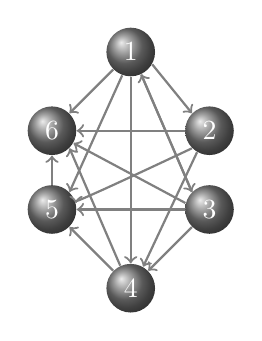
\begin{tikzpicture}
	\node[circle, shading=ball, ball color=gray, color=white] (1) at (0,2) {$1$};
	\node[circle, shading=ball, ball color=gray, color=white] (2) at (1,1) {$2$};
	\node[circle, shading=ball, ball color=gray, color=white] (3) at (1,0) {$3$};
	\node[circle, shading=ball, ball color=gray, color=white] (4) at (0,-1) {$4$};
	\node[circle, shading=ball, ball color=gray, color=white] (5) at (-1,0) {$5$};
	\node[circle, shading=ball, ball color=gray, color=white] (6) at (-1,1) {$6$};
	
	% vertex 1
	\draw[gray,->,thick](1) to [out=330,in=135,looseness=0](2);
	\draw[gray,->,thick](1) to [out=295,in=135,looseness=0](3);
	\draw[gray,->,thick](1) to [out=270,in=90,looseness=0](4);
	\draw[gray,->,thick](1) to [out=250,in=45,looseness=0](5);
	\draw[gray,->,thick](1) to [out=225,in=45,looseness=0](6);
	% vertex 2
	\draw[gray,->,thick](2) to [out=240,in=60,looseness=0](4);
	\draw[gray,->,thick](2) to [out=225,in=15,looseness=0](5);
	\draw[gray,->,thick](2) to [out=180,in=0,looseness=0](6);
	% vertex 3
	\draw[gray,->,thick](3) to [out=135,in=295,looseness=0](1);
	\draw[gray,->,thick](3) to [out=225,in=45,looseness=0](4);
	\draw[gray,->,thick](3) to [out=180,in=0,looseness=0](5);
	\draw[gray,->,thick](3) to [out=165,in=330,looseness=0](6);
	% vertex 4
	\draw[gray,->,thick](4) to [out=135,in=315,looseness=0](5);
	\draw[gray,->,thick](4) to [out=115,in=315,looseness=0](6);
	% vertex 5
	\draw[gray,->,thick](5) to [out=90,in=270,looseness=0](6);
	% vertex 6
\end{tikzpicture}%
}\hfill
&
\resizebox{0.2\textwidth}{!}{% Perturbed Random
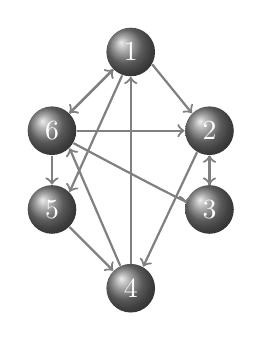
\begin{tikzpicture}
	\node[circle, shading=ball, ball color=gray, color=white] (1) at (0,2) {$1$};
	\node[circle, shading=ball, ball color=gray, color=white] (2) at (1,1) {$2$};
	\node[circle, shading=ball, ball color=gray, color=white] (3) at (1,0) {$3$};
	\node[circle, shading=ball, ball color=gray, color=white] (4) at (0,-1) {$4$};
	\node[circle, shading=ball, ball color=gray, color=white] (5) at (-1,0) {$5$};
	\node[circle, shading=ball, ball color=gray, color=white] (6) at (-1,1) {$6$};
	
	% vertex 1
	\draw[gray,->,thick](1) to [out=330,in=135,looseness=0](2);
	\draw[gray,->,thick](1) to [out=250,in=45,looseness=0](5);
	\draw[gray,->,thick](1) to [out=225,in=45,looseness=0](6);
	% vertex 2
	\draw[gray,->,thick](2) to [out=270,in=90,looseness=0](3);
	\draw[gray,->,thick](2) to [out=240,in=60,looseness=0](4);
	% vertex 3
	\draw[gray,->,thick](3) to [out=90,in=270,looseness=0](2);
	% vertex 4
	\draw[gray,->,thick](4) to [out=90,in=270,looseness=0](1);
	\draw[gray,->,thick](4) to [out=115,in=315,looseness=0](6);
	% vertex 5
	\draw[gray,->,thick](5) to [out=315,in=135,looseness=0](4);
	% vertex 6
	\draw[gray,->,thick](6) to [out=45,in=225,looseness=0](1);
	\draw[gray,->,thick](6) to [out=0,in=180,looseness=0](2);
	\draw[gray,->,thick](6) to [out=330,in=165,looseness=0](3);
	\draw[gray,->,thick](6) to [out=270,in=90,looseness=0](5);
\end{tikzpicture}%
}\hfill
&
\resizebox{0.2\textwidth}{!}{% Near Disconnected
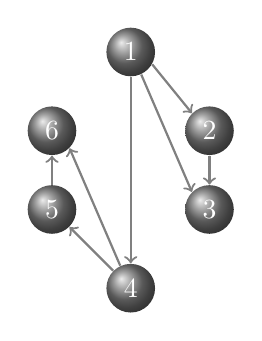
\begin{tikzpicture}
	\node[circle, shading=ball, ball color=gray, color=white] (1) at (0,2) {$1$};
	\node[circle, shading=ball, ball color=gray, color=white] (2) at (1,1) {$2$};
	\node[circle, shading=ball, ball color=gray, color=white] (3) at (1,0) {$3$};
	\node[circle, shading=ball, ball color=gray, color=white] (4) at (0,-1) {$4$};
	\node[circle, shading=ball, ball color=gray, color=white] (5) at (-1,0) {$5$};
	\node[circle, shading=ball, ball color=gray, color=white] (6) at (-1,1) {$6$};
	
	% vertex 1
	\draw[gray,->,thick](1) to [out=330,in=135,looseness=0](2);
	\draw[gray,->,thick](1) to [out=295,in=135,looseness=0](3);
	\draw[gray,->,thick](1) to [out=270,in=90,looseness=0](4);
	% vertex 2
	\draw[gray,->,thick](2) to [out=270,in=90,looseness=0](3);
	% vertex 3
	% vertex 4
	\draw[gray,->,thick](4) to [out=135,in=315,looseness=0](5);
	\draw[gray,->,thick](4) to [out=115,in=315,looseness=0](6);
	% vertex 5
	\draw[gray,->,thick](5) to [out=90,in=270,looseness=0](6);
	% vertex 6
\end{tikzpicture}%
}\\
$\specr = 1.0000$ & $\specr = 0.9382$ & $\specr = 0.7767$ & $\specr = 0.6000$ \\
$\ipr = 1.0000$ & $\ipr = 0.9996$ & $\ipr = 0.9987$ & $\ipr = 0.9930$ \\
& & & \\
\textbf{Random} & \textbf{Cycle} & \textbf{Completely Connected} & \textbf{Empty} \\
\resizebox{0.2\textwidth}{!}{% Random
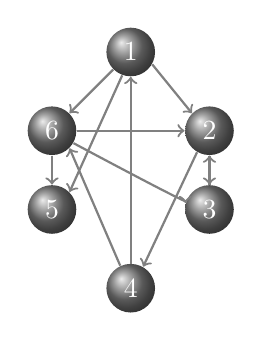
\begin{tikzpicture}
	\node[circle, shading=ball, ball color=gray, color=white] (1) at (0,2) {$1$};
	\node[circle, shading=ball, ball color=gray, color=white] (2) at (1,1) {$2$};
	\node[circle, shading=ball, ball color=gray, color=white] (3) at (1,0) {$3$};
	\node[circle, shading=ball, ball color=gray, color=white] (4) at (0,-1) {$4$};
	\node[circle, shading=ball, ball color=gray, color=white] (5) at (-1,0) {$5$};
	\node[circle, shading=ball, ball color=gray, color=white] (6) at (-1,1) {$6$};
	
	% vertex 1
	\draw[gray,->,thick](1) to [out=330,in=135,looseness=0](2);
	\draw[gray,->,thick](1) to [out=250,in=45,looseness=0](5);
	\draw[gray,->,thick](1) to [out=225,in=45,looseness=0](6);
	% vertex 2
	\draw[gray,->,thick](2) to [out=270,in=90,looseness=0](3);
	\draw[gray,->,thick](2) to [out=240,in=60,looseness=0](4);
	% vertex 3
	\draw[gray,->,thick](3) to [out=90,in=270,looseness=0](2);
	% vertex 4
	\draw[gray,->,thick](4) to [out=90,in=270,looseness=0](1);
	\draw[gray,->,thick](4) to [out=115,in=315,looseness=0](6);
	% vertex 5
	% vertex 6
	\draw[gray,->,thick](6) to [out=0,in=180,looseness=0](2);
	\draw[gray,->,thick](6) to [out=330,in=165,looseness=0](3);
	\draw[gray,->,thick](6) to [out=270,in=90,looseness=0](5);
\end{tikzpicture}%
}\hfill
&
\resizebox{0.2\textwidth}{!}{% Cycle
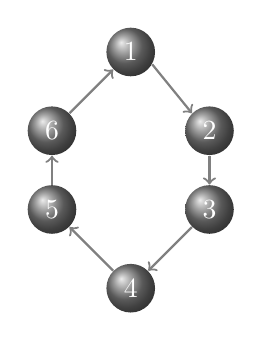
\begin{tikzpicture}
	\node[circle, shading=ball, ball color=gray, color=white] (1) at (0,2) {$1$};
	\node[circle, shading=ball, ball color=gray, color=white] (2) at (1,1) {$2$};
	\node[circle, shading=ball, ball color=gray, color=white] (3) at (1,0) {$3$};
	\node[circle, shading=ball, ball color=gray, color=white] (4) at (0,-1) {$4$};
	\node[circle, shading=ball, ball color=gray, color=white] (5) at (-1,0) {$5$};
	\node[circle, shading=ball, ball color=gray, color=white] (6) at (-1,1) {$6$};
	
	% vertex 1
	\draw[gray,->,thick](1) to [out=330,in=135,looseness=0](2);
	% vertex 2
	\draw[gray,->,thick](2) to [out=270,in=90,looseness=0](3);
	% vertex 3
	\draw[gray,->,thick](3) to [out=225,in=45,looseness=0](4);
	% vertex 4
	\draw[gray,->,thick](4) to [out=135,in=315,looseness=0](5);
	% vertex 5
	\draw[gray,->,thick](5) to [out=90,in=270,looseness=0](6);
	% vertex 6
	\draw[gray,->,thick](6) to [out=45,in=225,looseness=0](1);
\end{tikzpicture}%
}\hfill
&
\resizebox{0.2\textwidth}{!}{% Completely Connected
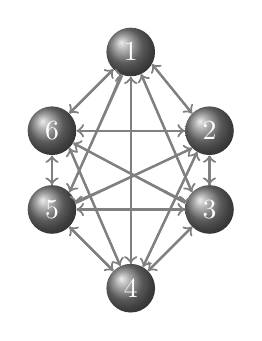
\begin{tikzpicture}
	\node[circle, shading=ball, ball color=gray, color=white] (1) at (0,2) {$1$};
	\node[circle, shading=ball, ball color=gray, color=white] (2) at (1,1) {$2$};
	\node[circle, shading=ball, ball color=gray, color=white] (3) at (1,0) {$3$};
	\node[circle, shading=ball, ball color=gray, color=white] (4) at (0,-1) {$4$};
	\node[circle, shading=ball, ball color=gray, color=white] (5) at (-1,0) {$5$};
	\node[circle, shading=ball, ball color=gray, color=white] (6) at (-1,1) {$6$};
	
	% vertex 1
	\draw[gray,->,thick](1) to [out=330,in=135,looseness=0](2);
	\draw[gray,->,thick](1) to [out=295,in=135,looseness=0](3);
	\draw[gray,->,thick](1) to [out=270,in=90,looseness=0](4);
	\draw[gray,->,thick](1) to [out=250,in=45,looseness=0](5);
	\draw[gray,->,thick](1) to [out=225,in=45,looseness=0](6);
	% vertex 2
	\draw[gray,->,thick](2) to [out=135,in=330,looseness=0](1);
	\draw[gray,->,thick](2) to [out=270,in=90,looseness=0](3);
	\draw[gray,->,thick](2) to [out=240,in=60,looseness=0](4);
	\draw[gray,->,thick](2) to [out=225,in=15,looseness=0](5);
	\draw[gray,->,thick](2) to [out=180,in=0,looseness=0](6);
	% vertex 3
	\draw[gray,->,thick](3) to [out=135,in=295,looseness=0](1);
	\draw[gray,->,thick](3) to [out=90,in=270,looseness=0](2);
	\draw[gray,->,thick](3) to [out=225,in=45,looseness=0](4);
	\draw[gray,->,thick](3) to [out=180,in=0,looseness=0](5);
	\draw[gray,->,thick](3) to [out=165,in=330,looseness=0](6);
	% vertex 4
	\draw[gray,->,thick](4) to [out=90,in=270,looseness=0](1);
	\draw[gray,->,thick](4) to [out=60,in=240,looseness=0](2);
	\draw[gray,->,thick](4) to [out=45,in=225,looseness=0](3);
	\draw[gray,->,thick](4) to [out=135,in=315,looseness=0](5);
	\draw[gray,->,thick](4) to [out=115,in=315,looseness=0](6);
	% vertex 5
	\draw[gray,->,thick](5) to [out=45,in=250,looseness=0](1);
	\draw[gray,->,thick](5) to [out=15,in=225,looseness=0](2);
	\draw[gray,->,thick](5) to [out=0,in=180,looseness=0](3);
	\draw[gray,->,thick](5) to [out=315,in=135,looseness=0](4);
	\draw[gray,->,thick](5) to [out=90,in=270,looseness=0](6);
	% vertex 6
	\draw[gray,->,thick](6) to [out=45,in=225,looseness=0](1);
	\draw[gray,->,thick](6) to [out=0,in=180,looseness=0](2);
	\draw[gray,->,thick](6) to [out=330,in=165,looseness=0](3);
	\draw[gray,->,thick](6) to [out=315,in=115,looseness=0](4);
	\draw[gray,->,thick](6) to [out=270,in=90,looseness=0](5);
\end{tikzpicture}%
}\hfill
&
\resizebox{0.2\textwidth}{!}{% Empty
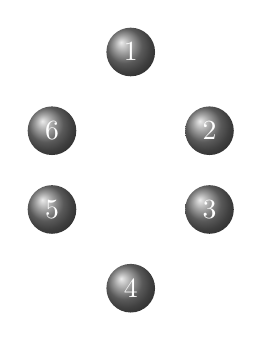
\begin{tikzpicture}
	\node[circle, shading=ball, ball color=gray, color=white] (1) at (0,2) {$1$};
	\node[circle, shading=ball, ball color=gray, color=white] (2) at (1,1) {$2$};
	\node[circle, shading=ball, ball color=gray, color=white] (3) at (1,0) {$3$};
	\node[circle, shading=ball, ball color=gray, color=white] (4) at (0,-1) {$4$};
	\node[circle, shading=ball, ball color=gray, color=white] (5) at (-1,0) {$5$};
	\node[circle, shading=ball, ball color=gray, color=white] (6) at (-1,1) {$6$};
	
	% vertex 1
	% vertex 2
	% vertex 3
	% vertex 4
	% vertex 5
	% vertex 6
\end{tikzpicture}%
}\\
$\specr = 0.6298$ & $\specr = 0.3000$ & $\specr = 0.2000$ & $\specr = 0.0000$ \\
$\ipr = 0.9900$ & $\ipr = 0.2700$ & $\ipr = 0.0000$ & $\ipr = 0.0000$.
\end{tabular}%
}
\caption{Structured graph data from~\cite{Anderson2018}.}
\label{fig:simod-examples}
\end{figure}

In Table~\ref{tab:big-east}, we record the rankability measure for each year of the NCAA Big East Football Conference from 1995 to 2012.
It is important to note that there is still a strong correlation to the rankability measure $\ipr$.
Moreover, there is a strong correlation to the predictability of Colley and Massey rankings~\cite{Colley2002,Massey1997}.
Hence, these rankability measures give a good indication of the inherent ability of the this data to produce a meaningful ranking of its items.
%%%%%%%%%%%%%%%%%%%%%%
%			Table 1				%
%%%%%%%%%%%%%%%%%%%%%%
\begin{table}
\centering
\begin{tabular}{|| c | c || c | c ||}
\hline
Year & $\specr$ & Year & $\specr$ \\
\hline
1995 & 0.8571 & 2004 & 0.6615\\
1996 & 0.8571 & 2005 & 0.8375\\
1997 & 0.8149 & 2006 & 0.8049\\
1998 & 0.8169 & 2007 & 0.6841\\
1999 & 0.8571 & 2008 & 0.8049\\
2000 & 0.8571 & 2009 & 0.8571\\
2001 & 0.8571 & 2010 & 0.7082\\ 
2002 & 0.8571 & 2011 & 0.7143\\
2003 & 0.8571 & 2012 & 0.7143\\
\hline
\end{tabular}
\caption{Big East Football Rankability}
\label{tab:big-east}
\end{table}

However, it is also clear from these measures that $\specr$ has trouble differentiation between certain years of the Big East data. 
This motivates our investigation of other graph properties that can be used to measure the rankability of data. 
In particular, we have used the algebraic connectivity of a graph to differentiate between years of the big east data and identify unique years as the least and most rankable. 
Now, our goal is to provide a rigorous theoretical justification for the use of the algebraic connectivity, just as was done with the spectral-degree characteristic in the Pre-Print. 

%%%%%%%%%%%%%%%%%%%%%%%%%%%%%%%%%%%%%%%%%%%%%%%%%%%%%%
%                                    				Algebraic Connectivity
%%%%%%%%%%%%%%%%%%%%%%%%%%%%%%%%%%%%%%%%%%%%%%%%%%%%%%
\section{Algebraic Connectivity}	
Let $\Gamma$ be a directed graph with non-negative weights and let $L$ be the graph Laplacian of $\Gamma$. 
Furthermore, let $e$ denote the all ones vector. 
Then, the algebraic connectivity of $L$ is defined as follows~\cite{Wu2005-1}:
\[
\alpha(\Gamma)=\min_{x\in S}x^{T}Lx,
\]
where
\[
S=\left\{x\in\mathbb{R}^{n}\colon x\perp e,\norm{x}=1\right\}.
\]
Another related and useful quantity is the following:
\[
\beta(\Gamma)=\max_{x\in S}x^{T}Lx.
\]
It is important to note that both $\alpha(\Gamma)$ and $\beta(\Gamma)$ are invariant under re-ordering of vertices of $\Gamma$ since the space $S$ is invariant under permutation. 

Let $Q$ be an orthonormal matrix whose columns span $S$.
Then, we have
\[
\alpha(\Gamma)=\min_{\norm{Qx}=1}x^{T}Q^{T}LQx
\]
and
\[
\beta(\Gamma)=\max_{\norm{Qx}=1}x^{T}Q^{T}LQx.
\]
Furthermore, let $F(A)$ denote the field of values of a complex matrix $A$, as defined in~\cite{Horn1991}.
Then, the Hermitian part of $A$, denoted $H(A)=\frac{1}{2}(A+A^{*})$, satisfies the following:
\[
F(H(A))=\re{F(A)}.
\]
Moreover, the end points of $\re{F(A)}$ are well-known to be the minimum and maximum eigenvalues of $H(A)$. 
Therefore, we have
\[
\alpha(\Gamma)=\lambda_{\text{min}}\left(\frac{1}{2}Q^{T}(L+L^{T})Q\right)
\]
and
\[
\beta(\Gamma)=\lambda_{\text{max}}\left(\frac{1}{2}Q^{T}(L+L^{T})Q\right).
\]

%%%%%%%%%%%%%%%%%%%%%%%%%%%%%%%%%%%%%%%%%%%%%%%%%%%%%%
%                                    				Basic Properties
%%%%%%%%%%%%%%%%%%%%%%%%%%%%%%%%%%%%%%%%%%%%%%%%%%%%%%
\subsection{Basic Properties}
One of the motivations for the definition of $\alpha(\Gamma)$ is the several properties of Fiedler's definition of the algebraic connectivity for undirected graphs that remain valid~\cite{Fiedler1973}.
For instance, we have the following super and sub additivity property.

%%%%%%%%%%%%%%%%%%%%%%
%			Proposition 2.1			%
%%%%%%%%%%%%%%%%%%%%%%
\begin{proposition}[See Lemma 1 of~\cite{Wu2005-1}]
If two graphs $\Gamma_{1}$ and $\Gamma_{2}$ have the same vertex set and disjoint edge sets, then
\[
\alpha(\Gamma_{1})+\alpha(\Gamma_{2})\leq\alpha(\Gamma_{1}\cup\Gamma_{2})\leq\beta_(\Gamma_{1}\cup\Gamma_{2})\leq\beta(\Gamma_{1})+\beta(\Gamma_{2}).
\]
\end{proposition}

We also have the following bounds that follow readily from the Courant-Fisher min-max theorem.

%%%%%%%%%%%%%%%%%%%%%%
%			Proposition 2.2			%
%%%%%%%%%%%%%%%%%%%%%%
\begin{proposition}
Denote the eigenvalues of the Hermitian part of $L$ by
\[
\lambda_{1}\leq\ldots\leq\lambda_{n}.
\]
Then, we have
\[
\lambda_{1}\leq\alpha(\Gamma)\leq\lambda_{2}
\]
and
\[
\lambda_{n-1}\leq\beta(\Gamma)\leq\lambda_{n}.
\]
\end{proposition}

%%%%%%%%%%%%%%%%%%%%%%
%			Theorem 2.3			%
%%%%%%%%%%%%%%%%%%%%%%
\begin{theorem}
Let $\Gamma$ be a perfect dominance graph.
Then,
\[
\beta(\Gamma)<n.
\]
\end{theorem}
\begin{proof}
Without loss of generality, we can assume that $L$ is in Frobenius normal form.
Then, the Hermitian part of $L$ satisfies
\[
H(L)=\begin{bmatrix} n-1 & -1/2 & \cdots & -1/2 \\
				-1/2 & n-2 & \cdots & -1/2 \\
				\vdots & & \ddots & \vdots \\
				-1/2 & -1/2 & \cdots & 0 \end{bmatrix}.
\]
Note that
\[
\lim_{k\rightarrow\infty}\left(\frac{1}{n}H(A)\right)^{k} < 1.
\]
Therefore, by Theorem 5.6.12 of~\cite{Horn2013}, the spectral norm satisfies
\[
\rho(H(A))<n,
\]
and the result follows from Proposition 2.2. 
\end{proof}

The following proposition aligns our definition of $\beta(\Gamma)$ for directed graphs with Fiedler's original definition for undirected graphs.

%%%%%%%%%%%%%%%%%%%%%%
%			Proposition 2.4			%
%%%%%%%%%%%%%%%%%%%%%%
\begin{proposition}[See Lemma 4 of~\cite{Wu2005-1}]
Let $\conj{\Gamma}$ denote the complement of $\Gamma$, which is obtained by reversing the direction of all the edges.
Then,
\[
\alpha(\Gamma)+\beta(\conj(\Gamma))=n.
\]
\end{proposition}

We also have the following connection between our definition of $\alpha(\Gamma)$ and Fiedler's original definition for undirected graphs as the second smallest eigenvalue of the graph Laplacian.

%%%%%%%%%%%%%%%%%%%%%%
%			Proposition 2.5			%
%%%%%%%%%%%%%%%%%%%%%%
\begin{proposition}[See Lemma 5 of~\cite{Wu2005-1}]
If $\lambda$ is an eigenvalue of $L$ not corresponding to the eigenvector $e$, then
\[
\alpha(\Gamma)\leq\re{\lambda}.
\]
\end{proposition}

%%%%%%%%%%%%%%%%%%%%%%
%			Theorem 2.6			%
%%%%%%%%%%%%%%%%%%%%%%
\begin{theorem}
Let $\Gamma$ be a perfect dominance graph.
Then,
\[
\alpha(\Gamma)\leq 1.
\]
\end{theorem}
\begin{proof}
Let $L$ be the graph Laplacian of $\Gamma$. 
By Theorem 3.2 of the attached pre-print, the eigenvalues of $L$ satisfy
\[
\sigma(L)=\left\{n-1,\ldots,1,0\right\},
\]
where $0$ is the only eigenvalue corresponding to the eigenvector $e$. 
The result follows from Proposition 2.5.
\end{proof}

We conclude this section with the following corollary.

%%%%%%%%%%%%%%%%%%%%%%
%			Corollary 2.7			%
%%%%%%%%%%%%%%%%%%%%%%
\begin{corollary}
Let $\Gamma$ be a perfect dominance graph.
Then,
\[
0<\alpha(\Gamma)\leq 1
~\text{ and }~
n-1\leq \beta(\Gamma) < n.
\]
\end{corollary}
\begin{proof}
Theorem 2.3 and Theorem 2.6 imply that
\[
\alpha(\Gamma)\leq 1
~\text{ and }~
\beta(\Gamma)<n.
\]
Furthermore, the reversal of a perfect dominance graph is also a perfect dominance graph.
In fact, $\conj{\Gamma}$ is a perfect dominance graph associated with the reverse ranking of $\Gamma$.
Hence $\conj{\Gamma}$ and $\Gamma$ are isomorphic and it follows that 
\[
\alpha(\Gamma)=\alpha(\conj{\Gamma})
~\text{ and }~
\beta(\Gamma)=\beta(\conj{\Gamma}).
\]
Therefore, Proposition 2.4 implies that
\[
\alpha(\Gamma)+\beta(\Gamma)=n.
\]
Hence,
\[
\alpha(\Gamma)=n-\beta(\Gamma)>0
\]
since $\beta(\Gamma)<n$. and
\[
\beta(\Gamma)=n-\alpha(\Gamma)\geq n-1
\]
since $\alpha(\Gamma)\leq 1$. 
\end{proof}

%%%%%%%%%%%%%%%%%%%%%%%%%%%%%%%%%%%%%%%%%%%%%%%%%%%%%%
%                                    				The Field of Values
%%%%%%%%%%%%%%%%%%%%%%%%%%%%%%%%%%%%%%%%%%%%%%%%%%%%%%
\subsection{The Field of Values}
We aspire to give a more specific description of $\alpha(\Gamma)$ and $\beta(\Gamma)$ when $\Gamma$ is a perfect dominance graph. 
Ideally, we would have a characterization result analogous to the spectral-degree characterization in Theorem 1.1. 
To this end, we have started an investigation of the field of values of the matrix $Q^{T}LQ$, where $Q$ is defined as in the beginning of Section 2.
After running some numerical experiments, the first thing we noticed is that $F(Q^{T}LQ)$ is an ellipse whenever $\Gamma$ is a perfect dominance graph.
In Figure 3, we display the field of values of $Q^{T}LQ$ for a perfect dominance graph on $3$, $6$, $9$, and $12$ vertices.

%%%%%%%%%%%%%%%%%%%%%%
%			Figure 3				%
%%%%%%%%%%%%%%%%%%%%%%
\begin{figure}[ht]
\centering
\begin{tabular}{cc}
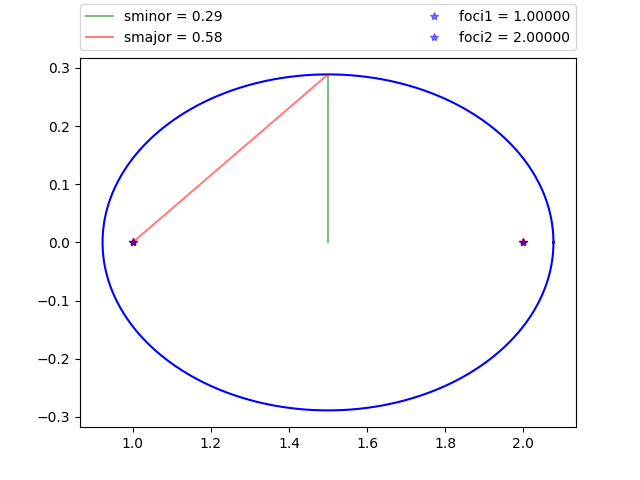
\includegraphics[width=0.45\textwidth]{figures/nr-dom-ellipse-3.png}
&
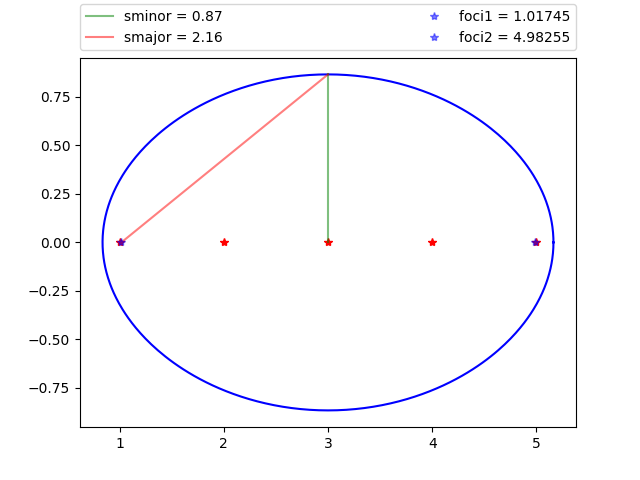
\includegraphics[width=0.45\textwidth]{figures/nr-dom-ellipse-6.png} \\
& \\
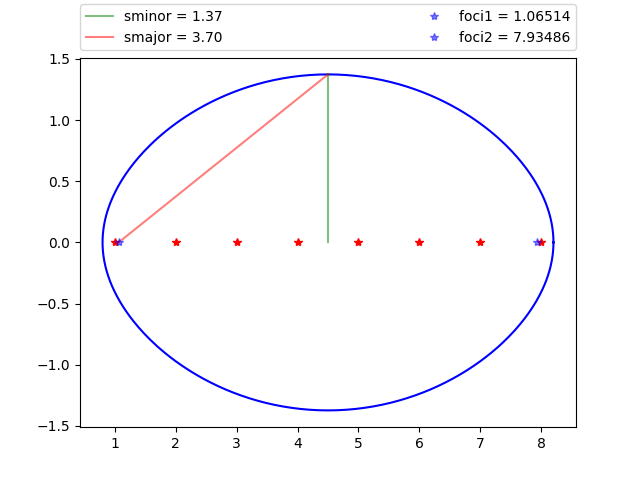
\includegraphics[width=0.45\textwidth]{figures/nr-dom-ellipse-9.png}
&
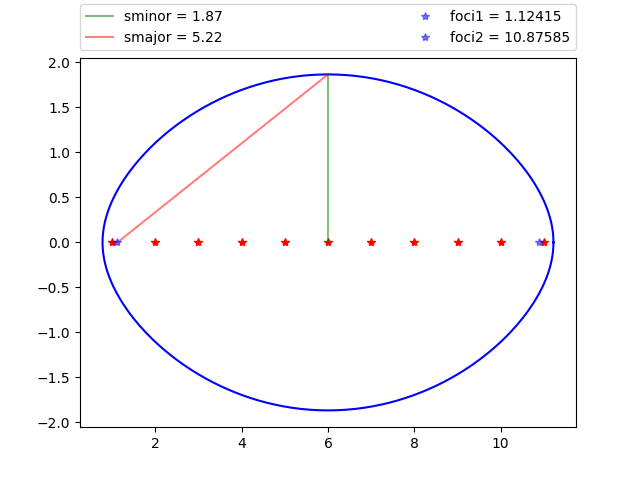
\includegraphics[width=0.45\textwidth]{figures/nr-dom-ellipse-12.png} \\
\end{tabular}
\caption{$F(Q^{T}LQ)$ for Perfect Dominance Graphs.}
\end{figure}

Note that for a perfect dominance graph on $3$ vertices, the matrix $Q^{T}LQ$ is $2\times 2$.
In particular, we have
\begin{align*}
Q^{T}LQ &= 
			\begin{bmatrix}1/\sqrt{2} & -1/\sqrt{2} & 0 \\
						1/\sqrt{6} & 1/\sqrt{6} & -2/\sqrt{6} \end{bmatrix}
			\begin{bmatrix} 2 & -1 & -1 \\
						0 & 1 & -1 \\
						0 & 0 & 0 \end{bmatrix}
			\begin{bmatrix}1/\sqrt{2} & 1/\sqrt{6} \\
					-1/\sqrt{2} & 1/\sqrt{6} \\
					0 & -2/\sqrt{6} \end{bmatrix} \\
		&= \begin{bmatrix}2 & 0 \\ 1/\sqrt{3} & 1 \end{bmatrix}.
\end{align*}
The eigenvalues of $Q^{T}LQ$ are
\[
\lambda_{1}=1~\text{ and }~\lambda_{2}=2.
\]
Furthermore, the singular values of $Q^{T}LQ$ are
\[
\sigma_{1} = \sqrt{\frac{2}{3}\left(4+\sqrt{7}\right)}
~\text{ and }~
\sigma_{2} = \sqrt{\frac{2}{3}\left(4-\sqrt{7}\right)}
\]
Therefore, by the elliptical range theorem, $F(Q^{T}LQ)$ is an ellipse with foci at $1$ and $2$, and with a major axis of length $\sqrt{16/3 - 1 - 4}\approx 0.58$. 

%%%%%%%%%%%%%%%%%%%%%%%%%%%%%%%%%%%%%%%%%%%%%%%%%%%%%%
%                                 	   			Bibliography
%%%%%%%%%%%%%%%%%%%%%%%%%%%%%%%%%%%%%%%%%%%%%%%%%%%%%%
\label{Bibliography}
\bibliographystyle{siam}
\bibliography{Bibliography}

\end{document}